\subsection{《第三种黑猩猩》}
谁能回答下列3个问题:世界上大部分纸浆,是以哪10种树木供应的?那10种树木,每一种有哪10种鸟为它清理害虫,哪10种昆虫为它传粉,哪10种动物为它散播种子?这10种鸟、昆虫、动物依赖哪些其他的物种?如果你是一个木材公司的总裁,想知道哪一个树种就算灭绝了也不会造成公司的损失,你就必须能够回答那3个不可能的问题。

雨林面积只占地表的6\% ,却蕴藏着地球生物圈一半物种

鸟类既容易观察又容易辨识,况且赏鸟人士很多。结果,所有动物中,我们对鸟类知道得最多。

动物在没有人的情境中演化,遇上了人之后,温驯而无惧。

工业革命以前的社会,几千年来一直在消灭物种,摧毁栖境,破坏自己的生存。

人类由猿类演化出来后,食性改变了,越来越依赖狩猎果腹。但是,我们的居住社群越来越大,社群成员的合作成为社群存亡的关键,人类于是演化出抑制杀戮冲动的本能。人类在漫长的演化史上,使用的武器有效范围都不远,适于近战,因此只要我们“不忍”下手杀害面前的敌人,就足以维系社群。使用现代武器,只需要挂钮(扣扳机),我们不必看且看清敌人的面孔,根本不会触动先前演化出来的抑制机制。于是,技术解放了人类的杀戮冲动(本能),劳心者(而非劳力者——“黑手”)策划/执行的“灭族屠杀”就登场了, 
\begin{figure}[htpb]
	\centering
	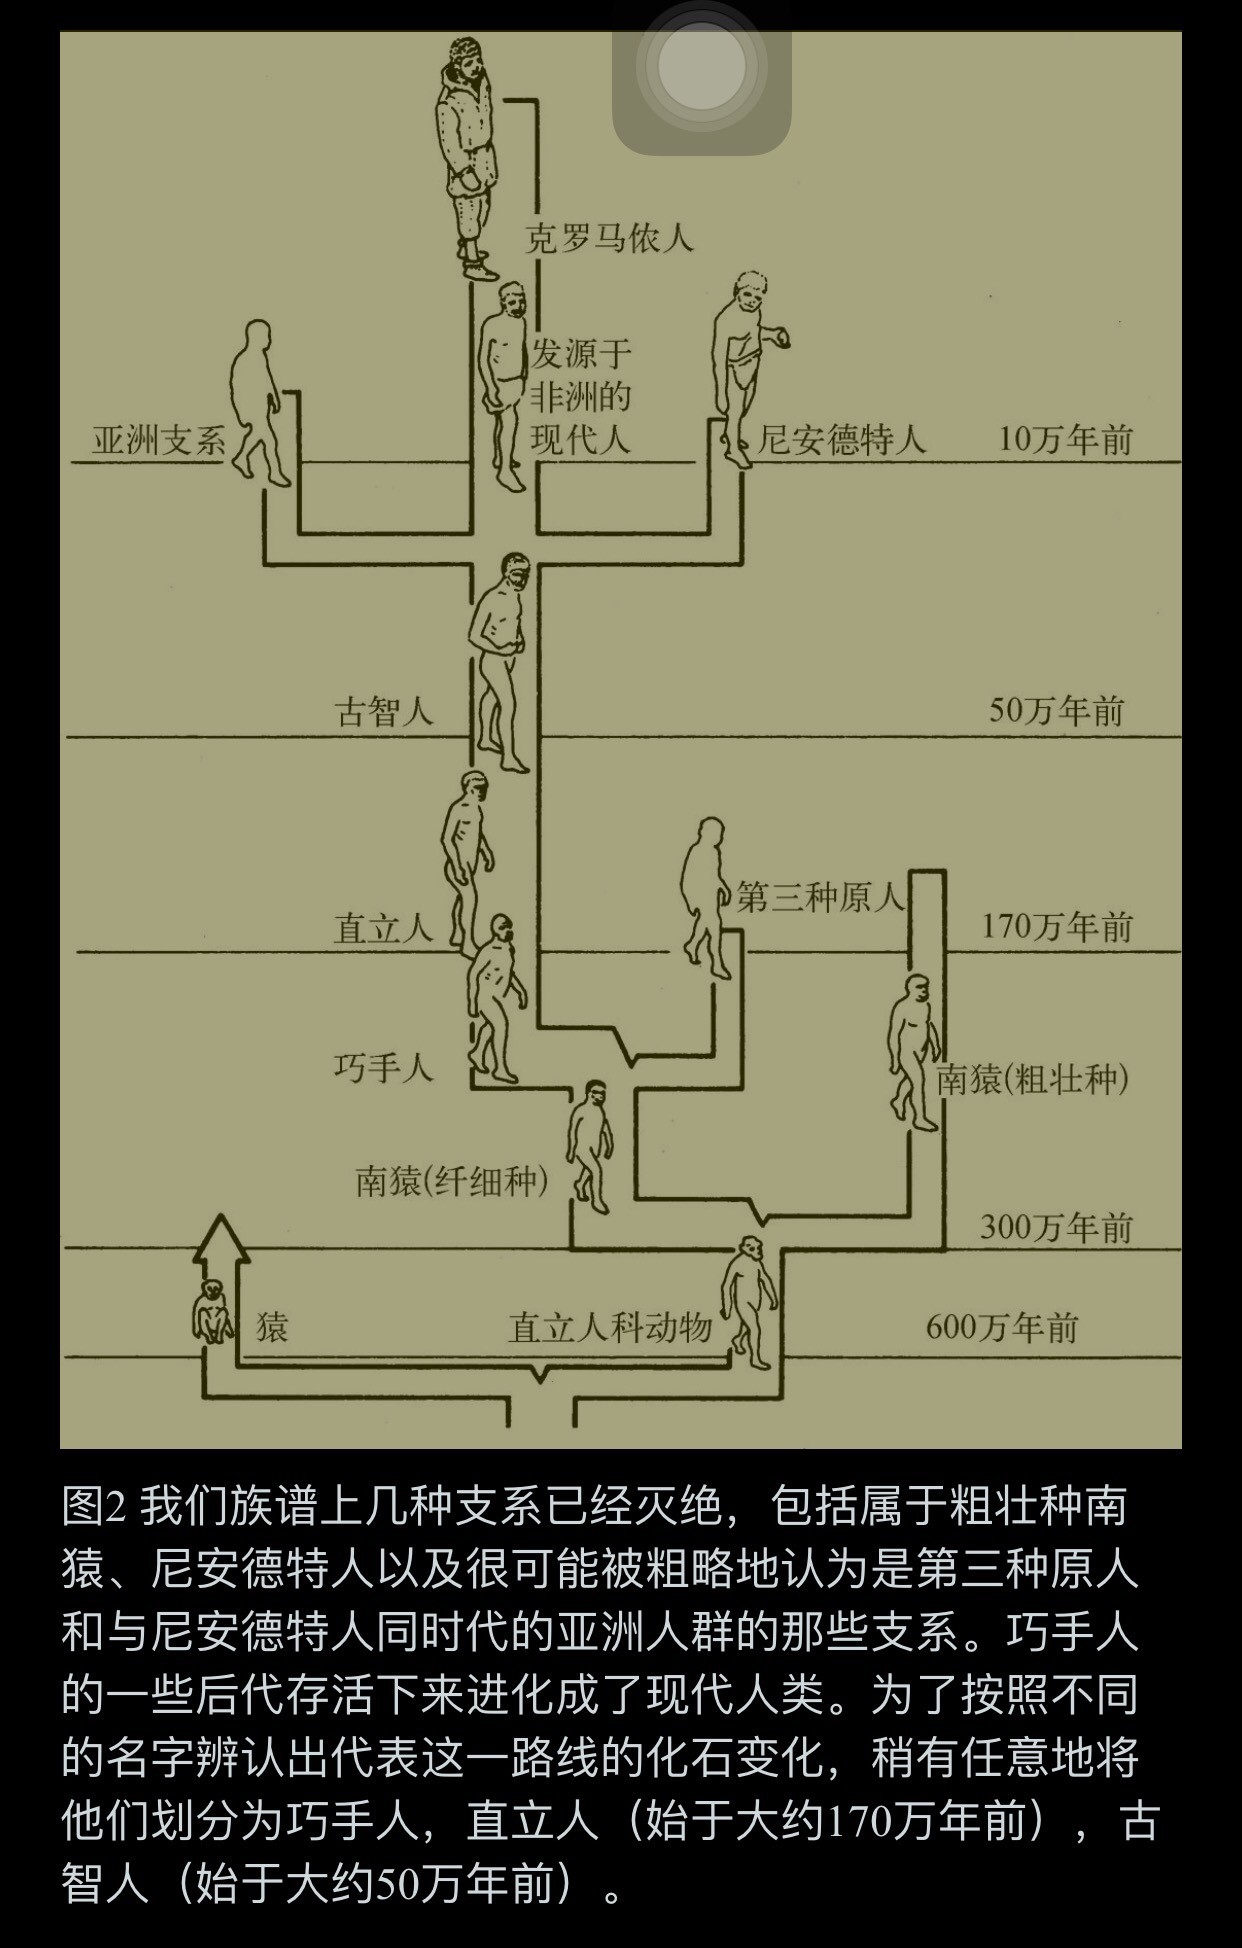
\includegraphics[width=0.6\linewidth]{images/hxx.jpg}
\end{figure}

在1917年,学者已经知道公元前1900年到公元前1500年间,世界上有两个印欧语系支系——安纳托利亚语与印度伊朗语。第三个支系是在1952年发现的古希腊文——“线性文字B”(Linear B)。其实“线性文字B”早就发现了,只是一直无法破解。那些“线性文字B”字板大约是公元前1300年的文物。

语言的演化有两个方面:一是世代变化,一是空间分化。

那些有害的身体构造与行为,构成了有效的指标,显示发出讯号的个体是诚实的:正因为那些形质特征或行为特征令个体陷于残障的境地,所以那个个体必然是优越的。不需花费成本就能发出的讯号,容易用来欺骗受讯的一方,因为跑得慢的、基因品质低劣的个体,都能发出那个讯号。只有高成本的、有害的讯号,才能保证诚实。

相关系数最高的项目(约正0.9)是:宗教、族裔、人种、社会经济条件、年龄与政治观点。

对于挑选伴侣,女人挑剔,男人随缘。

男人雄伟的阴茎,是威胁其他男人用的,或向其他男人炫耀自己地位的玩意儿。

我们的平均“交接”时间,大约是4分钟(美国人),大猩猩是1分钟,波诺波猿15秒,黑猩猩7秒,可是红毛猩猩可达15分钟,而比起袋鼠类(12小时),人类的表现“如露亦如电”。

阴茎勃起后的平均长度:大猩猩3.18厘米;红毛猩猩3.81厘米;黑猩猩7.62厘米;人类12.7厘米。视觉上的突出程度,也是同样的顺序:大猩猩的阴茎即使勃起了也毫不起眼,因为是黑色的;黑猩猩的阴茎勃起后呈粉红色,由于背景是无毛的白色皮肤,所以非常抢眼。雄猿的阴茎若不勃起,根本看不见。

性交次数频繁的物种,睾丸比较大;“杂交”的物种,雄性经常有轮番上阵与同一雌性性交的阵仗,特别需要大的睾丸(因为射精量最多的雄性使雌性怀孕的几率最大)。

雄性娶老婆最多的物种,通常是雄性身材比雌性大很多的物种。

大约发生在300万年前,当时人类家族分化为两个支系:一个支系是头骨粗壮、颊齿巨大的粗壮南猿;另一个支系,是头骨纤细一点、牙齿也较小的非洲南猿。